\documentclass[11pt]{article}

% ---------- fonts & math ----------
\usepackage[T1]{fontenc}
\usepackage[utf8]{inputenc}
\usepackage{mathpazo}
\linespread{1.06}

% ---------- layout ----------
\usepackage[letterpaper,margin=1in]{geometry}
\usepackage{titlesec}
\usepackage{parskip}
\setlength{\parskip}{0.45em plus 0.1em minus 0.1em}
\setlength{\parindent}{0pt}
\raggedbottom

% ---------- math tools ----------
\usepackage{amsmath}
\usepackage{amssymb}
\usepackage{mathtools}

% ---------- color, boxes, tables, figures ----------
\usepackage{xcolor}
\definecolor{accent}{HTML}{A13D2C}
\definecolor{accent2}{HTML}{2B5F6B}
\definecolor{muted}{HTML}{5A564F}
\definecolor{panel}{HTML}{F2EEE3}
\definecolor{linecol}{HTML}{D8D2C4}
\definecolor{ink}{HTML}{1E1C1A}
\color{ink}

\usepackage[most]{tcolorbox}
\tcbset{
  basestyle/.style={
    enhanced, breakable, colback=panel, colframe=linecol,
    boxrule=0.4pt, leftrule=2.4pt, arc=1.5pt, outer arc=1.5pt,
    left=10pt, right=10pt, top=7pt, bottom=7pt,
    fonttitle=\bfseries\sffamily\footnotesize,
    coltitle=muted, before skip=10pt, after skip=12pt
  },
  notebox/.style={basestyle, colframe=accent2},
  flagbox/.style={basestyle, colframe=accent}
}

\usepackage{booktabs}
\usepackage{array}
\usepackage{graphicx}
\graphicspath{{figs/}}
\usepackage{enumitem}
\usepackage{placeins}
\setlist[itemize]{leftmargin=1.4em, itemsep=0.35em, topsep=0.3em}

\usepackage{titling}
\usepackage[colorlinks=true, linkcolor=accent2, citecolor=accent2, urlcolor=accent2]{hyperref}

% ---------- section styling ----------
\titleformat{\section}
  {\normalfont\Large\bfseries}{\thesection}{0.6em}{}
\titlespacing{\section}{0pt}{1.6em}{0.8em}
\titleformat{\subsection}
  {\normalfont\large\bfseries\color{accent}}{}{0em}{}
\titlespacing{\subsection}{0pt}{1.1em}{0.4em}

\newcommand{\regime}[1]{\subsection*{#1}}

% ---------- title ----------
\title{\bfseries Signal, Noise, and Detection in CCD Photometry}
\author{}
\date{}

\begin{document}
\begin{center}
{\LARGE\bfseries Signal, Noise, and Detection in CCD Photometry}\\[6pt]
{\itshape\color{muted} A first-principles account of where the noise in a CCD measurement comes from,
how it sets the signal-to-noise ratio, and what that implies for how you should actually plan an exposure.}
\end{center}
\vspace{4pt}
\hrule
\vspace{14pt}

A CCD does not hand you a flux. It hands you a number of electrons collected in a set of pixels over
some time, and that number carries an uncertainty. Everything that matters observationally --- whether
an object is detected, how precisely its magnitude is known, whether it is smarter to take one long
exposure or many short ones --- follows from tracking that uncertainty honestly from its physical
origin down to the final signal-to-noise ratio, $\mathrm{SNR}$. That is the whole content of these
notes: no empirical fudge factors, just Poisson statistics applied to four physically distinct sources
of electrons, added the way independent random variables are supposed to be added.

\section*{Notation used throughout}

One deliberate choice, kept consistent for the rest of the document: every noise term is called
$\sigma$ (a standard deviation), never $N$ --- because $N$ is also the natural symbol for a photon
count, and reusing it for both ``count'' and ``noise'' is a standing source of confusion. Rates are
all called $R$ with a descriptive subscript, and the exposure is split into $N_{\rm exp}$ repeats of
length $t_{\rm exp}$ rather than the instrument-jargon NDIT/DIT.

\begin{center}
\begin{tabular}{@{}l p{9.4cm} l@{}}
\toprule
\textbf{Symbol} & \textbf{Meaning} & \textbf{Units} \\
\midrule
$R_{\rm src}$ & electron rate from the source, integrated over the photometric aperture & $\mathrm{e^-\,s^{-1}}$ \\
$R_{\rm sky}$ & sky-background electron rate, per pixel & $\mathrm{e^-\,s^{-1}\,pix^{-1}}$ \\
$R_{\rm dark}$ & dark-current electron rate, per pixel & $\mathrm{e^-\,s^{-1}\,pix^{-1}}$ \\
$n_{\rm pix}$ & number of pixels in the photometric aperture ($\propto \mathrm{seeing}^2$) & pixels \\
$t_{\rm exp}$, $N_{\rm exp}$ & duration of one exposure; number of exposures & s\ ;\ --- \\
$t = N_{\rm exp}\,t_{\rm exp}$ & total exposure time & s \\
$S = R_{\rm src}\,t$ & total signal: source electrons collected & $\mathrm{e^-}$ \\
$\sigma_{\rm RON}$ & read noise, per pixel per readout & $\mathrm{e^-}$ \\
$\sigma_x$ & standard deviation (``noise'') contributed by process $x$ & $\mathrm{e^-}$ \\
$\mathrm{SNR} = S/\sigma_{\rm tot}$ & signal-to-noise ratio & --- \\
$m$, $\delta m$ & magnitude; uncertainty on the magnitude & mag \\
\bottomrule
\end{tabular}
\end{center}

\section*{Setting up the measurement}

A photon hitting the detector is converted to a photoelectron with some probability $\eta$, the
quantum efficiency (typically $\eta \sim 0.5$--$0.85$ for a CCD). We will not carry $\eta$ around
explicitly: since it multiplies every photon rate by the same constant factor, we agree from the
outset to count everything in \emph{detected electrons}, and let $\eta$ be absorbed into the rates.
This is a bookkeeping choice, not a physical assumption --- but it means every rate below ($R_{\rm src}$,
$R_{\rm sky}$, $R_{\rm dark}$) is already ``post-QE.''

Over a total exposure time $t$, the source deposits a total signal
\begin{equation}
S = R_{\rm src}\, t .
\end{equation}
In practice $t$ is built out of $N_{\rm exp}$ individual exposures of length $t_{\rm exp}$ each:
\begin{equation}
t = N_{\rm exp}\, t_{\rm exp}, \qquad S = R_{\rm src}\, N_{\rm exp}\, t_{\rm exp}.
\end{equation}
This distinction --- total time $t$ versus how it is \emph{partitioned} into $N_{\rm exp}$ chunks ---
turns out to be the whole story later, because some noise terms care only about $t$ and one cares
specifically about $N_{\rm exp}$.

\section*{What noise buys you: from SNR to an error bar on the magnitude}

The noise $\sigma$ is the $1\sigma$ uncertainty on $S$: a measurement is reported as $S \pm \sigma$.
The signal-to-noise ratio is defined as
\begin{equation}
\mathrm{SNR} = \frac{S}{\sigma_{\rm tot}},
\end{equation}
so $1/\mathrm{SNR}$ is just the fractional uncertainty on the measurement. It is the single number
that tells you how much you can trust what you measured:

\begin{center}
\begin{tabular}{@{}l l p{7.2cm}@{}}
\toprule
\textbf{SNR} & \textbf{fractional error $1/\mathrm{SNR}$} & \textbf{what it means} \\
\midrule
2--3 & 33--50\% & object barely detected \\
5 & 20\% & detected --- you can believe you're seeing something real \\
10 & 10\% & a real measurement \\
100 & 1\% & excellent \\
\bottomrule
\end{tabular}
\end{center}

Because astronomers report brightness in magnitudes rather than flux, it is worth converting once and
for all. By definition $m = -2.5\log_{10}(S)$ (up to zero-point constants that don't depend on $S$ and
therefore drop out of any error propagation). If the true count deviates from $S$ by the noise
$\sigma$, the induced shift in magnitude is
\begin{equation}
\delta m \;=\; 2.5\log_{10}\!\left(\frac{S+\sigma}{S}\right) \;=\; 2.5\log_{10}\!\left(1+\frac{\sigma}{S}\right).
\end{equation}
For $\sigma/S \ll 1$ this linearizes ($\ln(1+x)\approx x$) to the familiar rule of thumb
\begin{equation}
\delta m \;\approx\; \frac{2.5}{\ln 10}\cdot\frac{\sigma}{S} \;=\; \frac{1.0857}{\mathrm{SNR}}.
\label{eq:dmag-approx}
\end{equation}

\begin{tcolorbox}[notebox, title=CHECKED NUMERICALLY]
The exact expression (Eq.~4) and the linear approximation (Eq.~5) agree well at high SNR but diverge
once the fractional error becomes large --- exactly where a linearization should be expected to fail.
The comparison in Fig.~1 confirms the rule of thumb $\delta m \sim 1/\mathrm{SNR}$ is safe once SNR is
above about 10, but at $\mathrm{SNR}=2$--3 (barely detected) the exact logarithmic form should be used
instead.
\end{tcolorbox}

\begin{figure}[htbp]
\centering
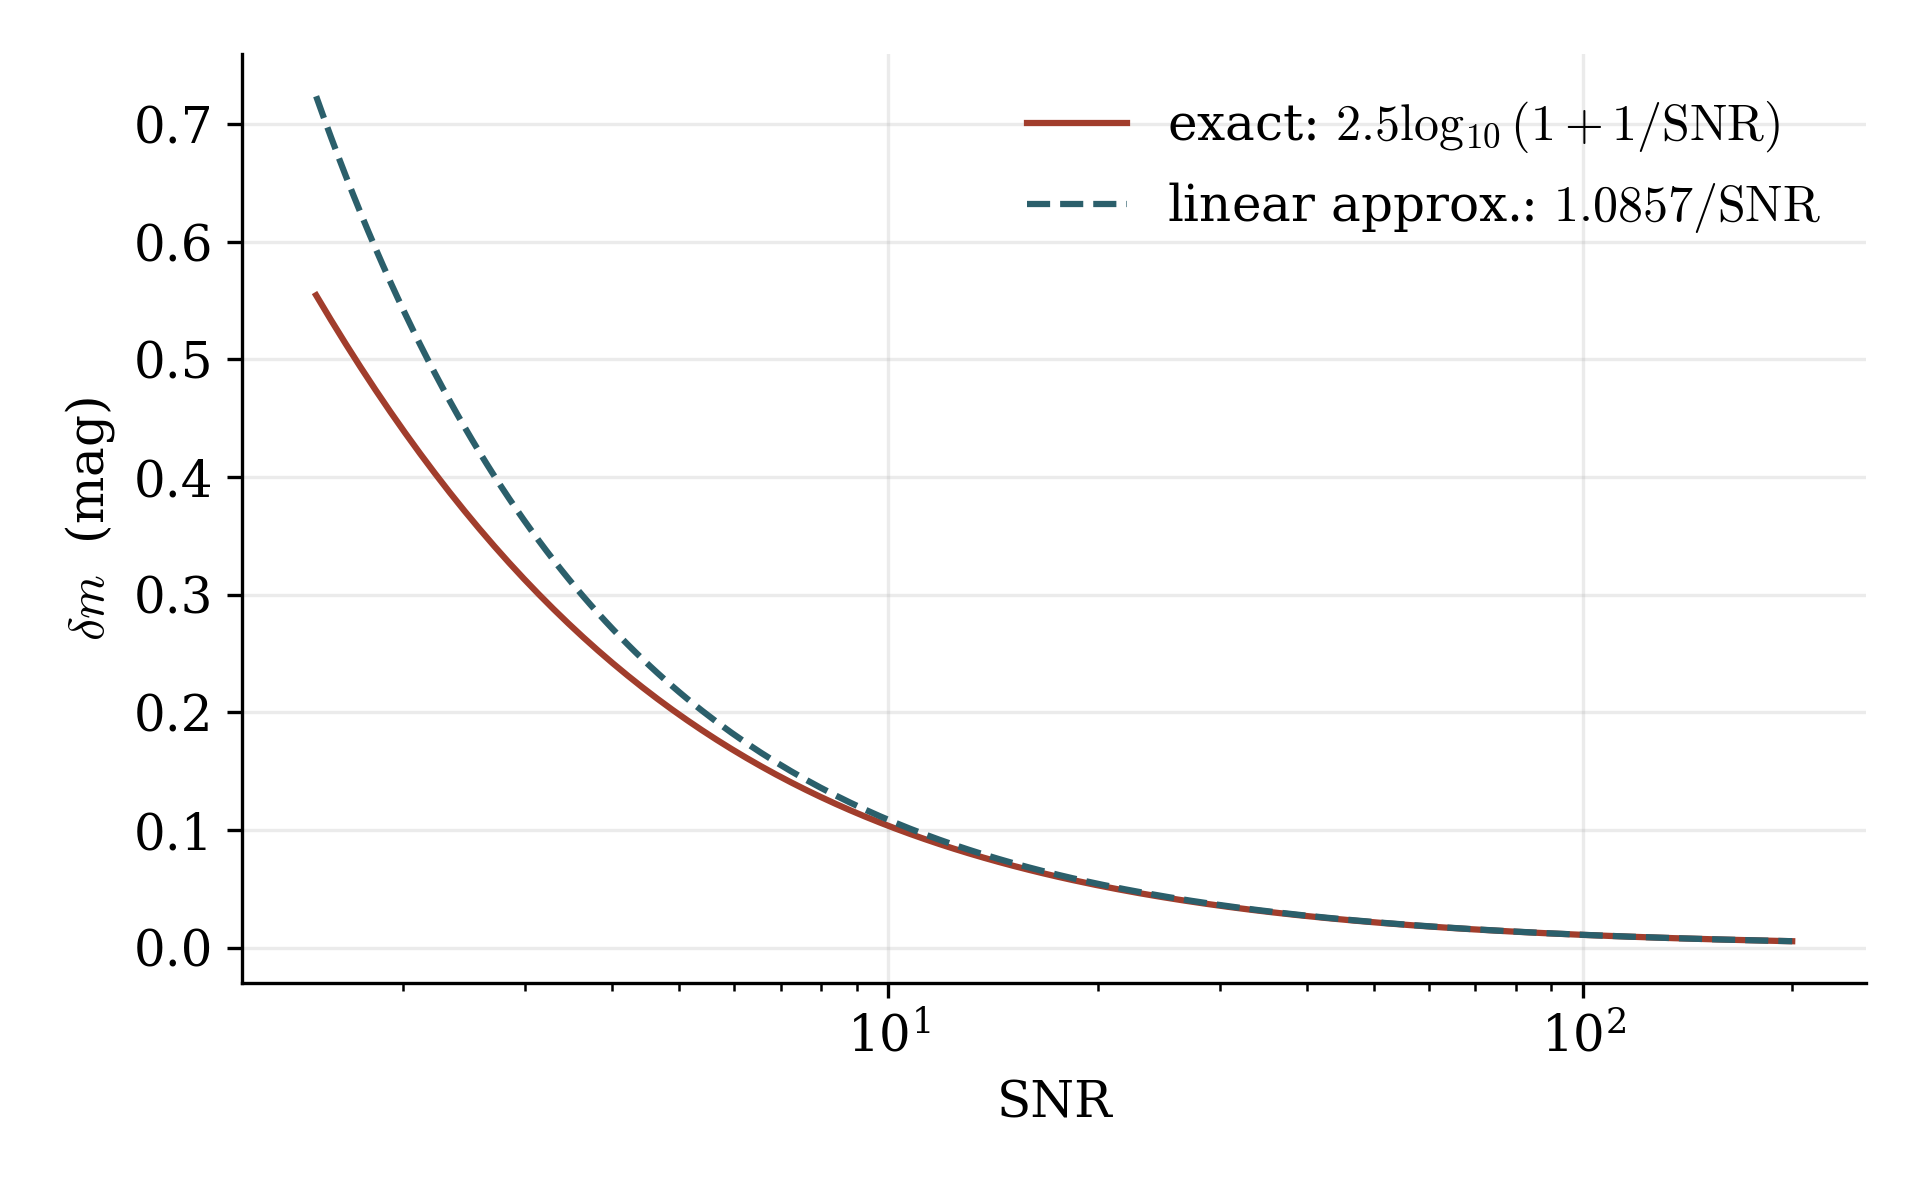
\includegraphics[width=0.72\textwidth]{figs/fig3_dmag.png}
\caption{Exact magnitude error versus the linear small-error approximation, as a function of SNR. The
two curves are indistinguishable above $\mathrm{SNR}\sim20$ and diverge below $\mathrm{SNR}\sim5$.}
\end{figure}

These numbers are not an arbitrary convention, and it's worth pausing to justify them rather than
just citing the table. The table actually answers two different questions, and its two halves answer
different ones: rows 2--3 and 5 answer ``is this real, or could it just be noise?''; rows 10 and 100
answer ``given that it's real, how precisely do I know its brightness?'' They happen to share the same
axis (SNR) because both questions are governed by the same ratio, but the reasoning behind each is
worth making explicit.

\subsection*{Rows 2--3 and 5: SNR as a detection significance}

\textbf{Assumption.} The total noise $\sigma_{\rm tot}$ is well approximated by a Gaussian
(normal) distribution. This is a genuinely new assumption, not a repeat of the Poisson assumption
from the next section --- but it is a well justified one: $\sigma_{\rm tot}$ is built from a sum
of many independent contributions (electrons from many photons, many pixels, many reads), and the
Central Limit Theorem says that a sum of many independent random contributions tends toward a
Gaussian regardless of the shape of the individual distributions, provided no single term dominates
the sum. (A single Poisson variable itself becomes Gaussian at large $\mu$, since its skewness scales
as $1/\sqrt{\mu}$ and vanishes as $\mu$ grows.) This is precisely what licenses treating ``SNR'' as a
literal number of standard deviations, i.e.\ speaking of a ``$k\sigma$ detection.''

With that assumption in hand, pose the question precisely: suppose that, in truth, there is no object
at this location --- the real signal is $S=0$, and every electron measured is background and noise.
The measured count still fluctuates, by construction, with standard deviation $\sigma_{\rm tot}$
around zero. The probability that noise alone produces an apparent excess of at least $k\sigma_{\rm
tot}$ is the upper tail of the Gaussian,
\begin{equation}
P(k) = \int_{k}^{\infty}\frac{1}{\sqrt{2\pi}}e^{-x^2/2}\,dx = 1-\Phi(k),
\label{eq:falsealarm}
\end{equation}
where $\Phi$ is the standard normal CDF. Because $\mathrm{SNR}=k$ in this hypothetical no-signal case,
Eq.~\ref{eq:falsealarm} converts an observed SNR directly into a \emph{false-alarm probability}: the
chance that what you're looking at is pure noise dressed up to look like a detection.

\begin{tcolorbox}[notebox, title=CHECKED NUMERICALLY]
Evaluating Eq.~\ref{eq:falsealarm} numerically:
$P(2)=2.3\times10^{-2}$ (1 in 44), $P(3)=1.4\times10^{-3}$ (1 in 741),
$P(5)=2.9\times10^{-7}$ (1 in 3.5 million), $P(10)=7.6\times10^{-24}$. The probability falls by roughly
an order of magnitude or more with each extra unit of $k$ --- Fig.~2 shows the full curve.
\end{tcolorbox}

\begin{figure}[htbp]
\centering
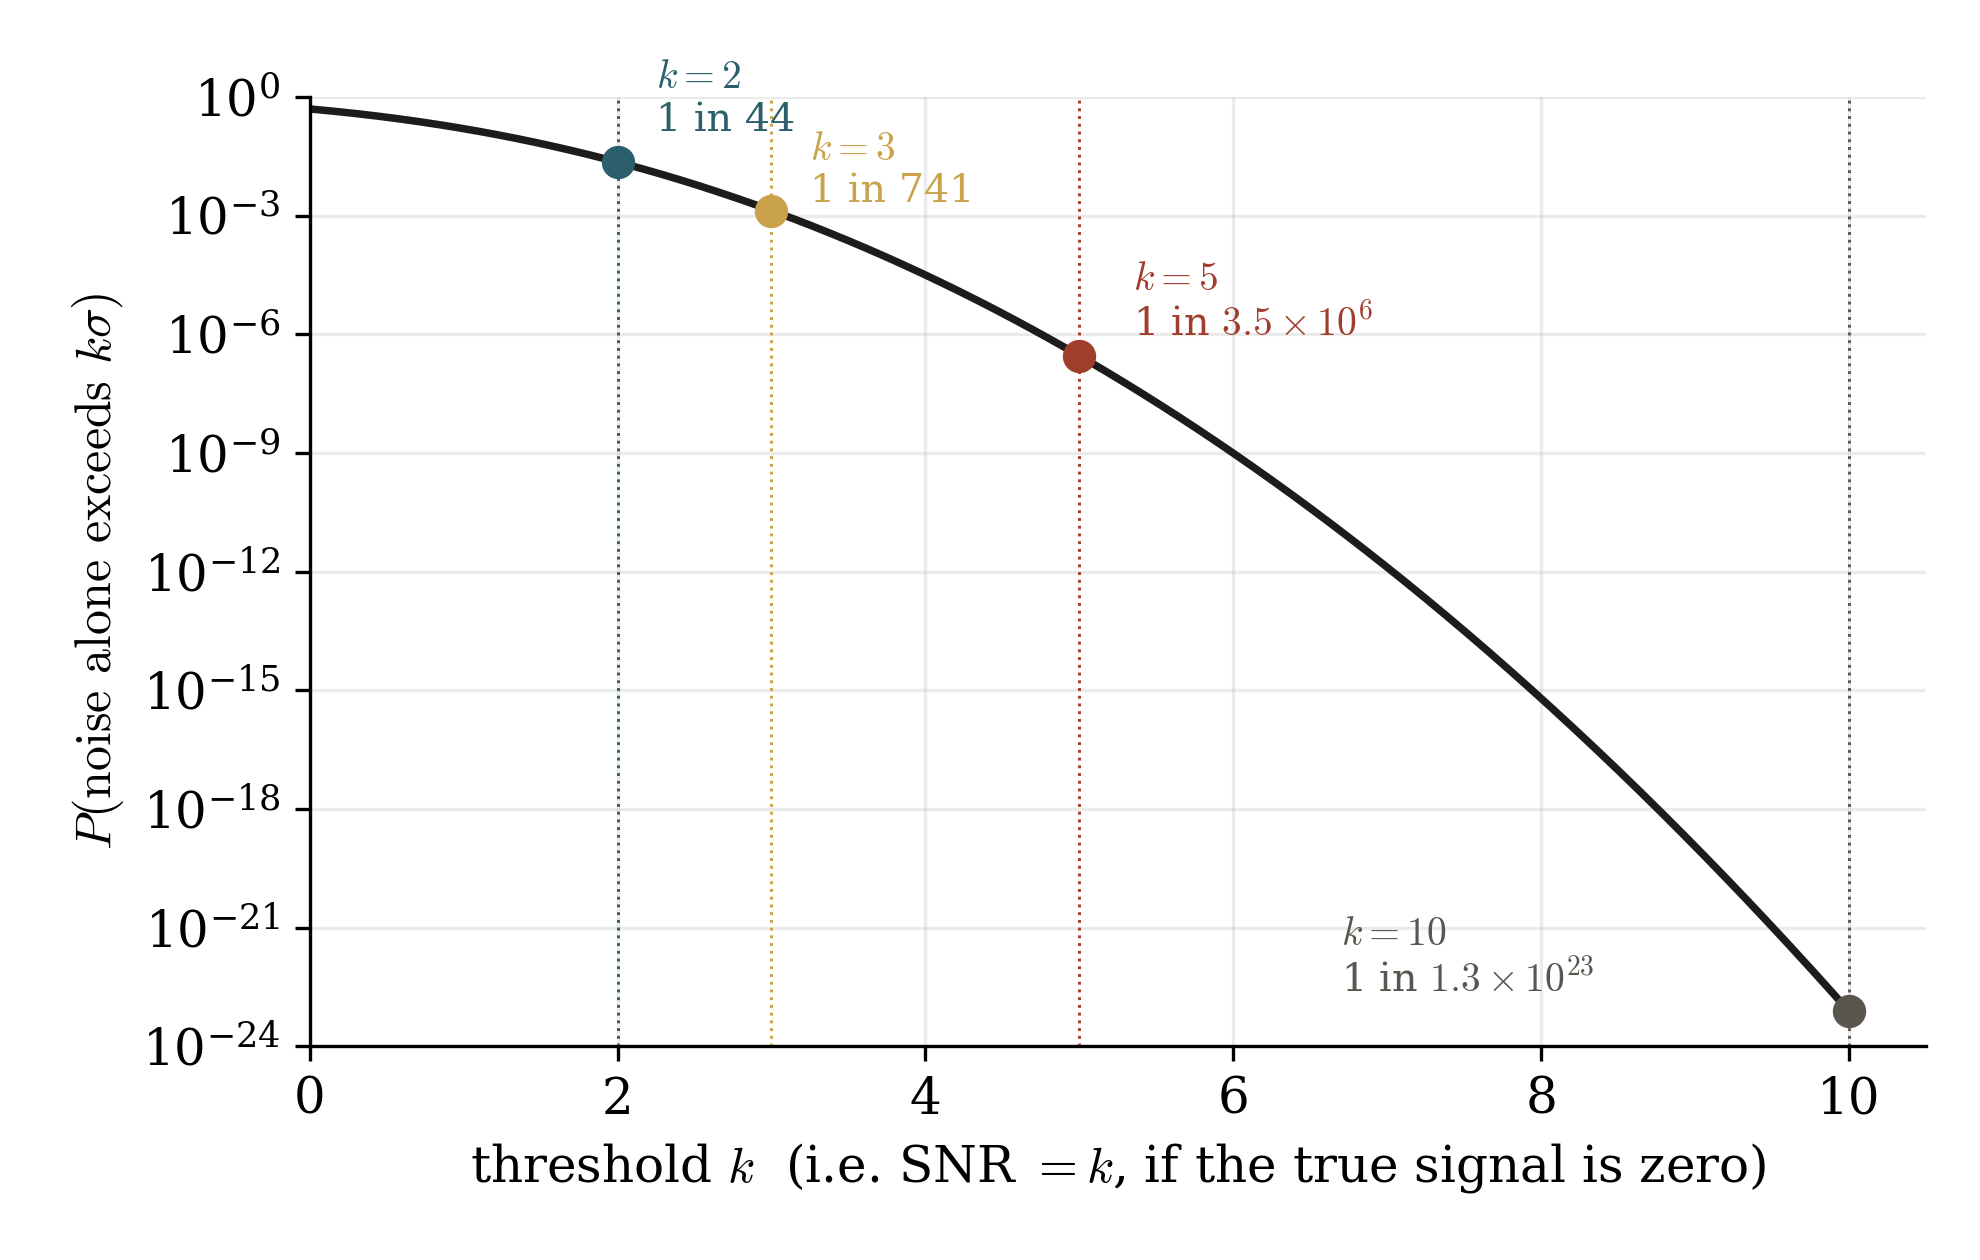
\includegraphics[width=0.72\textwidth]{figs/fig_gaussian_tail.png}
\caption{The probability that noise alone (Gaussian, mean zero) produces an apparent excess of at
least $k\sigma$, plotted on a log scale, for the case of a single pre-specified measurement. This is
exactly why $\mathrm{SNR}=2$--3 is only ``barely'' trusted (there is still a percent-level chance
it's a fluctuation) while $\mathrm{SNR}=5$ is treated as essentially certain: a one-in-3.5-million
fluke is not a serious competing explanation.}
\end{figure}

This is enough to explain rows 2--3 and 5 \emph{for a single, pre-chosen measurement} --- checking the
brightness of one specific, already-known star, say. But an important qualification is needed before
this reasoning is complete.

\begin{tcolorbox}[flagbox, title=THE CATCH: FALSE ALARMS MULTIPLY WITH THE NUMBER OF TRIES]
Eq.~\ref{eq:falsealarm} is a \emph{per-trial} probability. If instead of checking one pre-chosen
location you scan an entire image of $n_{\rm trial}$ independent pixels or apertures looking for
whatever turns up (a blind search for new sources), the chance that \emph{at least one} of them
exceeds the threshold by chance alone is, for small $P(k)$, approximately
\begin{equation}
P_{\rm any}(k) \approx n_{\rm trial}\,P(k)
\end{equation}
(a union bound: the probability of at least one rare event among many independent tries is
approximately the sum of the individual probabilities). For a $4000\times4000$ image,
$n_{\rm trial}=1.6\times10^7$, and at $k=3$ the expected number of pure-noise ``detections'' is
$n_{\rm trial}P(3)\approx 2.2\times10^4$ --- utterly swamped by false positives, useless as a blind
detection threshold. At $k=5$ the expectation drops to $\sim4.6$; by $k\approx5.5$--6 it is comfortably
below 1. This is exactly why blind searches (transient surveys, particle-physics discovery claims)
conventionally demand ``$5\sigma$'' rather than ``$3\sigma$'': the higher bar is not tradition for its
own sake, it is what keeps the expected count of noise-only false positives, summed over every one of
the many independent trials in the search, at or below about one. A targeted measurement of a single
known object is not a blind search --- it is one trial, not $n_{\rm trial}$ --- which is why the same
table casually lists $\mathrm{SNR}=2$--3 as ``barely detected'' rather than ``worthless'': it is
worthless \emph{as a blind-search claim}, but usable as a single, pre-registered check.
\end{tcolorbox}

\subsection*{Rows 10 and 100: SNR as a measurement precision}

By $\mathrm{SNR}=10$ the false-alarm probability from Eq.~\ref{eq:falsealarm} is already
astronomically small ($\sim10^{-24}$ at $k=10$, from the box above) --- so rows 10 and 100 are not
answering ``is it real?'' at all; that question is already settled. They answer a completely different
one: given that the object is real, how well do you know \emph{how bright} it is? That question is
answered directly by the fractional error $1/\mathrm{SNR}$ derived above, and by its magnitude-space
version, Eq.~\ref{eq:dmag-approx}: $\mathrm{SNR}=10$ means a $10\%$ flux error, about
$0.1\,\mathrm{mag}$ --- usable for a rough photometric point. $\mathrm{SNR}=100$ means $1\%$, about
$0.01\,\mathrm{mag}$ --- the level needed for precision work such as transit photometry or
millimag-level variability studies.

So the full table is really two different axes glued together by a shared symbol: the low end (2--3, 5)
is a statement about statistical confidence that a source exists at all (governed by Gaussian tail
probabilities, and secretly dependent on how many independent trials you searched over), while the
high end (10, 100) is a statement about how precisely you know its brightness once existence is no
longer in question (governed directly by $1/\mathrm{SNR}$, already derived above).


\section*{Where the noise actually comes from}

$\sigma$ is not one thing. It is the quadrature sum of several statistically independent
contributions, and the physics of each is different --- which is exactly why the answer to ``should I
take one long exposure or ten short ones?'' depends on which term dominates.

\subsection*{1. Shot noise: why counting photons is noisy even for a perfectly steady source}

Before writing down $\sigma=\sqrt{\mu}$, it's worth asking why there should be any noise at all in the
first place. If a star's true brightness is perfectly constant, why isn't the electron count perfectly
reproducible from one exposure to the next? The answer is that light is not a continuous fluid; it
arrives at the detector as a stream of discrete quanta (photons), and \emph{even a perfectly stable
source emits those quanta at random, independent times}. This randomness is not a flaw in the
instrument --- it is a property of the light itself, and no amount of engineering removes it. That
irreducible floor is what ``shot noise'' means (the name comes from the analogous effect in an
electrical current, which is carried by discrete electrons arriving at random times rather than by a
smooth flow of charge). Because it is fundamental rather than instrumental, it is the right place to
start: everything else in this section (sky, dark, read noise) is a variation on the same counting
argument, or, in the case of read noise, a genuinely different mechanism introduced for contrast.

\textbf{Assumption.} Photon arrivals from the source are independent of one another, and occur at a
constant mean rate $\lambda$ (photons per second) over the exposure. This is an excellent approximation
for essentially all classical (thermal or incoherent) astronomical sources; it is exactly the
statement that the light is \emph{not} correlated in a way that makes photons arrive in bunches or
avoid each other.

\textbf{From independent arrivals to a distribution.} Split the total exposure time $t$ into $N$ equal
subintervals of width $\Delta t = t/N$, with $N$ large enough that $\Delta t$ is small. In each
subinterval, the probability of detecting exactly one photon is $p = \lambda\,\Delta t$, and the
probability of detecting more than one vanishes as $\Delta t\to0$; so each subinterval is a Bernoulli
trial, and --- because the arrivals are independent by assumption --- the total count $n$ over all $N$
subintervals follows a Binomial distribution,
\begin{equation}
P(n) = \binom{N}{n}\,p^{\,n}(1-p)^{N-n}, \qquad p = \lambda\Delta t = \frac{\mu}{N},
\end{equation}
where $\mu \equiv \lambda t$ is the expected total count over the full exposure. Now take the limit
$N\to\infty$ (finer and finer subintervals) at fixed $\mu = Np$. Using
$N!/(N-n)! \to N^n$ and $(1-\mu/N)^{N-n}\to e^{-\mu}$ as $N\to\infty$, the binomial collapses to the
\emph{Poisson distribution}:
\begin{equation}
P(n;\mu) = \frac{\mu^{n}e^{-\mu}}{n!}.
\label{eq:poisson}
\end{equation}
This is the only distribution consistent with independent, constant-rate arrivals --- it is not an
extra assumption, it is a consequence of the one assumption already made above.

\textbf{Mean and variance, derived, not asserted.} The mean of Eq.~\ref{eq:poisson} is
\begin{equation}
\langle n\rangle = \sum_{n=0}^{\infty} n\,\frac{\mu^n e^{-\mu}}{n!}
= \mu e^{-\mu}\sum_{n=1}^{\infty}\frac{\mu^{n-1}}{(n-1)!}
= \mu e^{-\mu} e^{\mu} = \mu,
\end{equation}
where the sum was reindexed with $k=n-1$ and recognized as the exponential series. The same trick
applied to $n(n-1)$ gives the second factorial moment,
\begin{equation}
\langle n(n-1)\rangle = \sum_{n=0}^{\infty} n(n-1)\,\frac{\mu^n e^{-\mu}}{n!}
= \mu^2 e^{-\mu}\sum_{n=2}^{\infty}\frac{\mu^{n-2}}{(n-2)!} = \mu^2,
\end{equation}
so that $\langle n^2\rangle = \langle n(n-1)\rangle + \langle n\rangle = \mu^2+\mu$, and the variance is
\begin{equation}
\mathrm{Var}(n) = \langle n^2\rangle - \langle n\rangle^2 = \mu^2+\mu-\mu^2 = \mu.
\end{equation}
The mean and the variance of a Poisson variable are the same number, $\mu$ --- a special, non-obvious
property of this particular distribution, not a generic fact about randomness. The noise (standard
deviation) follows immediately:
\begin{equation}
\sigma = \sqrt{\mathrm{Var}(n)} = \sqrt{\mu}.
\end{equation}
This single relation, applied three times to three different electron sources (source, sky, dark
current, each its own independent Poisson process with its own $\mu$), generates three of the four
terms in the noise budget.

\begin{tcolorbox}[notebox, title=CHECKED NUMERICALLY]
For $\mu=10$, summing Eq.~\ref{eq:poisson} directly (truncated at $n=200$, far past where the terms
become negligible) gives $\sum_n P(n)=1.0000$, $\langle n\rangle = 10.000$, and
$\mathrm{Var}(n)=10.000$ --- confirming the closed-form results above rather than just asserting them.
\end{tcolorbox}

\begin{figure}[htbp]
\centering
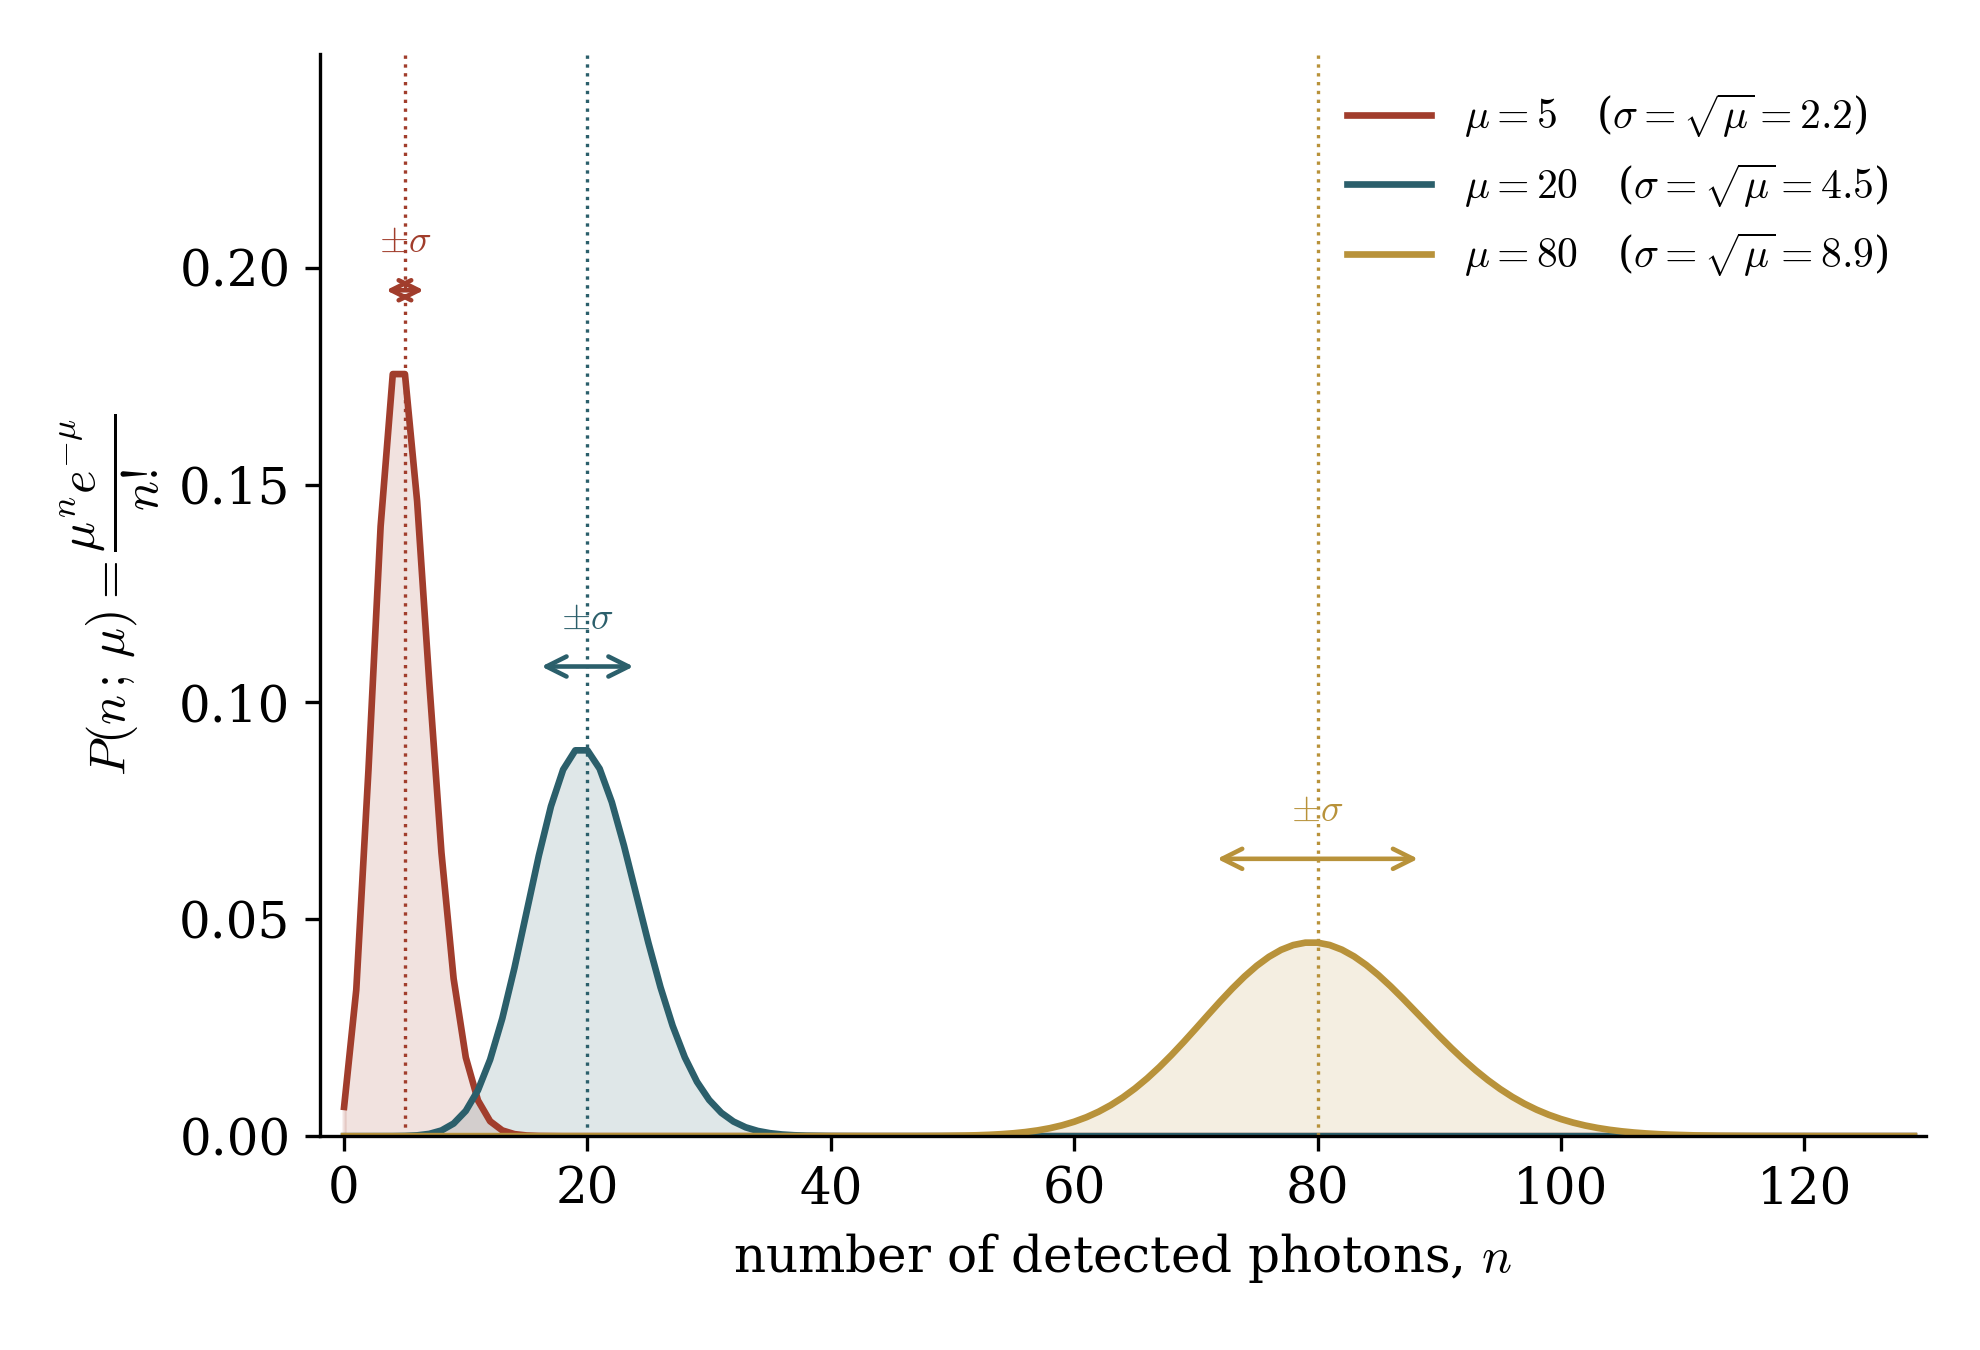
\includegraphics[width=0.82\textwidth]{figs/fig0_poisson.png}
\caption{The Poisson distribution $P(n;\mu)$ for three mean photon counts. The horizontal arrows mark
$\pm\sigma=\pm\sqrt{\mu}$ around each mean. Two things to read off directly: the \emph{absolute} width
grows with $\mu$ (a brighter source really does have a noisier raw count), while the width
\emph{relative to the mean}, $\sigma/\mu = 1/\sqrt{\mu}$, visibly shrinks --- the three curves get
narrower in proportion to their height as $\mu$ increases. This is precisely why $\mathrm{SNR}=\mu/\sigma=\sqrt{\mu}$
improves as you collect more light, and why it does so only as a square root rather than linearly: the
noise grows too, just more slowly than the signal.}
\end{figure}

\textbf{Object shot noise.} The object itself delivers $S = R_{\rm src}\,t$ electrons, and by the
Poisson rule above,
\begin{equation}
\sigma_{\rm src} = \sqrt{S} = \sqrt{R_{\rm src}\,t}.
\end{equation}

\textbf{Sky shot noise.} You cannot measure the object without also collecting sky background in the
same aperture, and that sky signal has to be estimated and subtracted --- but its own shot noise
cannot be subtracted away. With $R_{\rm sky}$ the sky rate per pixel and $n_{\rm pix}$ the number of
pixels in the photometric aperture (set by the seeing: $n_{\rm pix}\propto\mathrm{seeing}^2$), the
total sky electrons collected under the object are $n_{\rm pix}R_{\rm sky}\,t$, so
\begin{equation}
\sigma_{\rm sky} = \sqrt{n_{\rm pix}\,R_{\rm sky}\,t}.
\end{equation}

\textbf{Dark-current shot noise.} Thermal electrons generated inside the silicon itself, independent
of any light, accumulate at a rate $R_{\rm dark}$ per pixel, hence
\begin{equation}
\sigma_{\rm dark} = \sqrt{n_{\rm pix}\,R_{\rm dark}\,t}.
\end{equation}

\begin{tcolorbox}[flagbox, title=FLAGGING AN AMBIGUITY IN THE UNITS]
Dark current is often quoted per hour, purely because it's a small number over a typical exposure. But
$\sigma_{\rm dark}=\sqrt{n_{\rm pix}R_{\rm dark}\,t}$ is only dimensionally consistent if $R_{\rm dark}$
and $t$ use the \emph{same} time unit. If a data sheet gives $R_{\rm dark}$ in $\mathrm{e^-\,hr^{-1}}$
and $t$ is integrated in seconds, convert first: $R_{\rm dark}\,[\mathrm{e^-\,s^{-1}}] = R_{\rm dark}\,
[\mathrm{e^-\,hr^{-1}}]/3600$. Throughout these notes, $R_{\rm src}$, $R_{\rm sky}$, $R_{\rm dark}$ are
all per second, matching $t$ in seconds --- a convention made explicit here rather than left implicit.
\end{tcolorbox}

\subsection*{2. Read noise: not a shot-noise term}
Every time the chip is read out, the on-chip
amplifier adds a noise contribution $\sigma_{\rm RON}$ (electrons), fixed per pixel per readout,
independent of exposure time or flux. It doesn't come from counting anything, so it doesn't obey the
$\sqrt{\mu}$ scaling --- it is simply a fixed number added once per read. Reading $n_{\rm pix}$ pixels
once contributes noise $\sqrt{n_{\rm pix}}\,\sigma_{\rm RON}$ (independent per-pixel noises add in
quadrature). Reading out $N_{\rm exp}$ times over the course of building up the total exposure means
paying this penalty $N_{\rm exp}$ times:
\begin{equation}
\sigma_{\rm read} = \sqrt{n_{\rm pix}\,N_{\rm exp}}\;\;\sigma_{\rm RON}.
\end{equation}
This is the crucial structural difference from the three shot-noise terms:
$\sigma_{\rm read}^2 \propto N_{\rm exp}$, not $t$. Splitting a fixed total time into more
sub-exposures costs additional read noise, for free, every time.

\section*{Assembling the total: the master SNR equation}

\begin{tcolorbox}[notebox, title=FIRST-PRINCIPLES DERIVATION: WHY VARIANCES ADD FOR INDEPENDENT NOISE SOURCES]
Let $X$ and $Y$ be two random variables representing independent physical noise processes with expected values $\mu_X = \mathbb{E}[X]$, $\mu_Y = \mathbb{E}[Y]$ and variances $\sigma_X^2 = \mathrm{Var}(X)$, $\sigma_Y^2 = \mathrm{Var}(Y)$.

The variance of their sum $Z = X + Y$ is defined by:
\begin{equation}
\mathrm{Var}(X + Y) = \mathbb{E}\left[\big((X + Y) - \mathbb{E}[X + Y]\big)^2\right] = \mathbb{E}\left[\big((X - \mu_X) + (Y - \mu_Y)\big)^2\right].
\end{equation}
Expanding the algebraic square inside the expectation:
\begin{equation}
\big((X - \mu_X) + (Y - \mu_Y)\big)^2 = (X - \mu_X)^2 + (Y - \mu_Y)^2 + 2(X - \mu_X)(Y - \mu_Y).
\end{equation}
Applying the linearity of the mathematical expectation operator $\mathbb{E}[\,\cdot\,]$:
\begin{align}
\mathrm{Var}(X + Y) &= \mathbb{E}\left[(X - \mu_X)^2\right] + \mathbb{E}\left[(Y - \mu_Y)^2\right] + 2\,\mathbb{E}\left[(X - \mu_X)(Y - \mu_Y)\right] \notag \\
&= \mathrm{Var}(X) + \mathrm{Var}(Y) + 2\,\mathrm{Cov}(X, Y).
\end{align}
Because the physical mechanisms generating astronomical source photons, sky background photons, thermal dark current, and amplifier readout noise are statistically \emph{independent}, their joint probability density factorizes: $p(x, y) = p_X(x)\,p_Y(y)$. The covariance therefore vanishes identically:
\begin{equation}
\mathrm{Cov}(X, Y) = \mathbb{E}[(X - \mu_X)]\,\mathbb{E}[(Y - \mu_Y)] = 0 \cdot 0 = 0.
\end{equation}
By mathematical induction, for $N$ mutually independent noise contributions $X_1, X_2, \dots, X_N$:
\begin{equation}
\mathrm{Var}\left(\sum_{i=1}^N X_i\right) = \sum_{i=1}^N \mathrm{Var}(X_i) \quad\Longrightarrow\quad \sigma_{\rm tot}^2 = \sum_{i=1}^N \sigma_i^2 \quad\Longleftrightarrow\quad \sigma_{\rm tot} = \sqrt{\sum_{i=1}^N \sigma_i^2}.
\end{equation}
This rigorous result proves why independent noise contributions must be added in quadrature, establishing the fundamental basis of the CCD noise budget.
\end{tcolorbox}

Because the four contributions arise from independent physical processes, their variances add:
\begin{equation}
\sigma_{\rm tot}^2 = \sigma_{\rm src}^2 + \sigma_{\rm sky}^2 + \sigma_{\rm dark}^2 + \sigma_{\rm read}^2.
\end{equation}
Substituting the four expressions derived above,
\begin{tcolorbox}[enhanced, colback=white, colframe=ink, boxrule=0.9pt, arc=0pt,
                   left=14pt, right=14pt, top=10pt, bottom=10pt]
\begin{equation}
\mathrm{SNR} \;=\; \frac{R_{\rm src}\,t}
{\sqrt{\,R_{\rm src}\,t \;+\; n_{\rm pix}R_{\rm sky}\,t \;+\; n_{\rm pix}R_{\rm dark}\,t \;+\; n_{\rm pix}N_{\rm exp}\,\sigma_{\rm RON}^2\,}}
\label{eq:master}
\end{equation}
\end{tcolorbox}
with $t = N_{\rm exp}t_{\rm exp}$. Every quantity here is a property of the target ($R_{\rm src}$), the
sky ($R_{\rm sky}$), the instrument ($n_{\rm pix}$, $R_{\rm dark}$, $\sigma_{\rm RON}$), or the
observing strategy ($t$, $N_{\rm exp}$). This is the formula an exposure-time calculator evaluates;
everything below is what it looks like in the three limits where one term wins.

\begin{figure}[htbp]
\centering
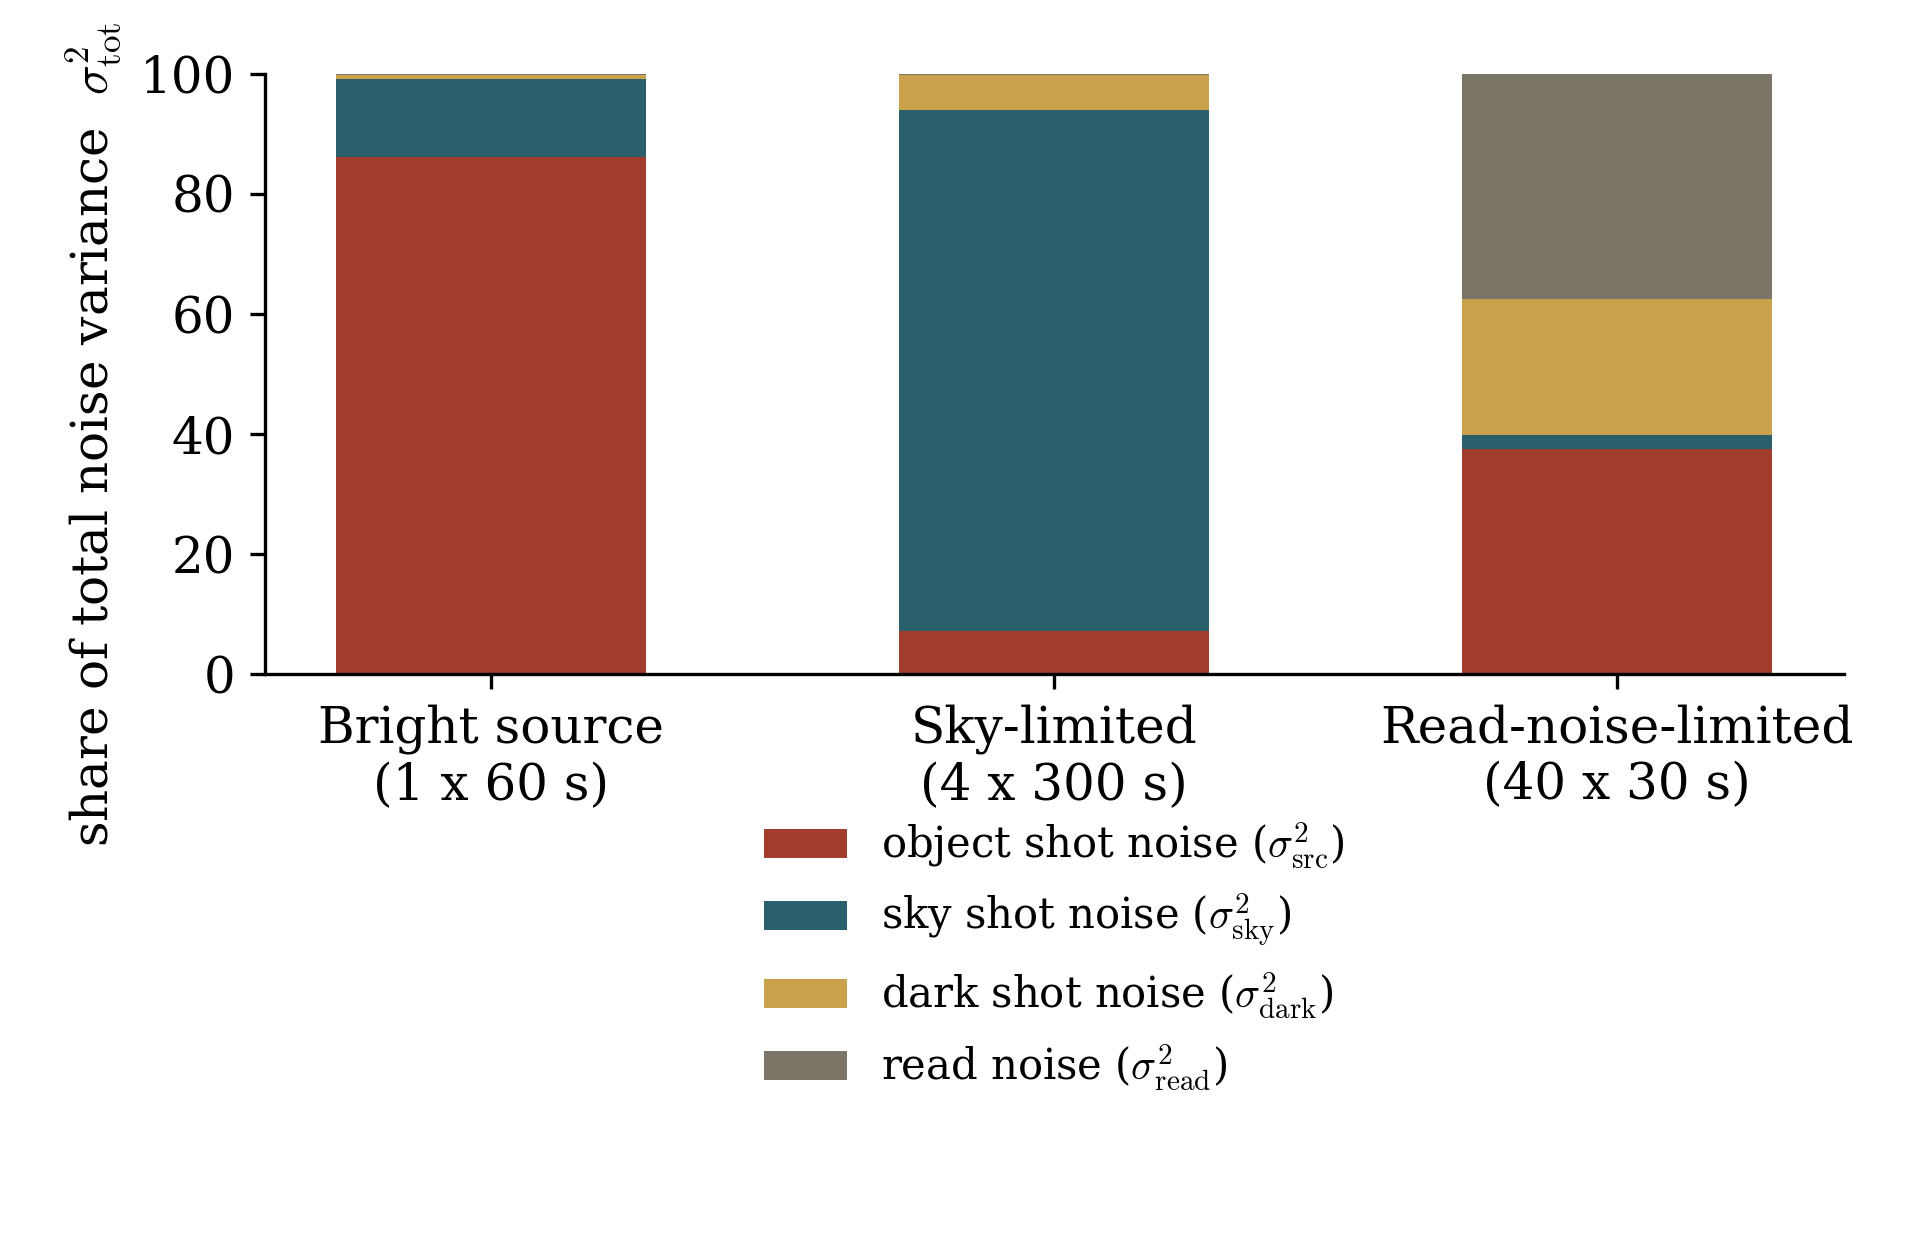
\includegraphics[width=0.85\textwidth]{figs/fig1_budget.png}
\caption{The four variance terms of the master equation, normalized to sum to 100\%, evaluated for
three representative setups (parameters chosen to be illustrative, not from a specific instrument).
This is exactly what ``which regime am I in?'' means in practice: look at which slice dominates.}
\end{figure}


\section*{The three regimes, and why they dictate how you observe}

\regime{Bright source (photon / shot-noise limited)}
When the target is bright enough that $R_{\rm src}\,t$ swamps sky, dark, and read noise, the master
equation collapses to
\begin{equation}
\mathrm{SNR} = \frac{R_{\rm src}t}{\sqrt{R_{\rm src}t}} = \sqrt{R_{\rm src}t}
\quad\Longrightarrow\quad \mathrm{SNR}\propto\sqrt{t}.
\end{equation}
This is the regime of bright standard stars: the practical limit is not reaching adequate SNR but
avoiding saturation of the detector.

\regime{Sky-background limited}
For a faint object against a bright sky, $R_{\rm sky}\gg R_{\rm src}$, so the sky term dominates the
sum under the square root:
\begin{equation}
\mathrm{SNR} \approx \frac{R_{\rm src}t}{\sqrt{n_{\rm pix}R_{\rm sky}t}}
\quad\Longrightarrow\quad \mathrm{SNR}\propto\frac{\sqrt{t}}{\sqrt{n_{\rm pix}}}.
\end{equation}
Two consequences follow directly, and both are operationally important:
\begin{itemize}
\item Since $n_{\rm pix}\propto\mathrm{seeing}^2$, tighter seeing (smaller effective aperture) directly
buys SNR --- this is why image quality matters even when you're not resolution-limited scientifically.
\item SNR depends only on the \emph{total} time $t=N_{\rm exp}t_{\rm exp}$, not on how it is split. One
3000\,s exposure and ten 300\,s exposures give (to first order) the same SNR, provided each
sub-exposure is individually sky-dominated. In practice, splitting is usually the better choice anyway
--- it lets you reject cosmic rays and build a better flat field --- and it costs essentially nothing.
\end{itemize}
This is the regime of broadband optical imaging and low-resolution optical spectroscopy, and --- in a
more extreme form --- near-infrared imaging, where the sky is so bright that long individual exposures
would saturate the array within seconds; there, splitting into many short exposures is not a choice
but a necessity, and the physics above says it's harmless to SNR.

\regime{Read-noise limited}
When sky and dark are both small (narrow-band imaging, high-resolution or echelle spectroscopy, where
the light per pixel is intrinsically low), the read-noise term wins:
\begin{equation}
\mathrm{SNR} \approx \frac{R_{\rm src}t}{\sqrt{n_{\rm pix}N_{\rm exp}}\,\sigma_{\rm RON}}
\quad\Longrightarrow\quad \mathrm{SNR}\propto\frac{1}{\sqrt{n_{\rm pix}}}\cdot\frac{1}{\sqrt{N_{\rm exp}}}.
\end{equation}
Here the two factors give two distinct, actionable levers:
\begin{itemize}
\item \textbf{Binning.} $n_{\rm pix}$ is the number of pixels actually \emph{read out}, not an
immutable property of the source. Binning $2\times2$ on-chip before readout reduces $n_{\rm pix}$ by a
factor of 4 and hence buys a factor $\sqrt{4}=2$ in SNR --- genuinely free signal-to-noise, at the cost
of spatial (or spectral) resolution. Keep at least $\sim2$ binned pixels across the seeing disk
(imaging) or across a spectral line (spectroscopy); binning past that throws away resolution you
needed.
\item \textbf{Minimize $N_{\rm exp}$.} Since $\mathrm{SNR}\propto N_{\rm exp}^{-1/2}$ at fixed total
time, $t_{\rm exp}$ should be as long as possible (equivalently $N_{\rm exp}$ as small as possible)
--- the opposite strategy from the sky-limited case. The practical ceiling on $t_{\rm exp}$ is usually
set by cosmic-ray accumulation (commonly $\sim$45\,min for CCDs), not by any noise term in this
equation; if cosmic rays genuinely don't matter to the science, there's no formal reason not to go
longer still.
\end{itemize}
This regime governs narrow-band imaging (sky reduced to a couple of electrons per pixel, exposures up
to $\sim$1\,hr) and echelle spectroscopy, where light is dispersed over so many resolution elements
that the sky contribution per pixel becomes negligible.

\begin{figure}[htbp]
\centering
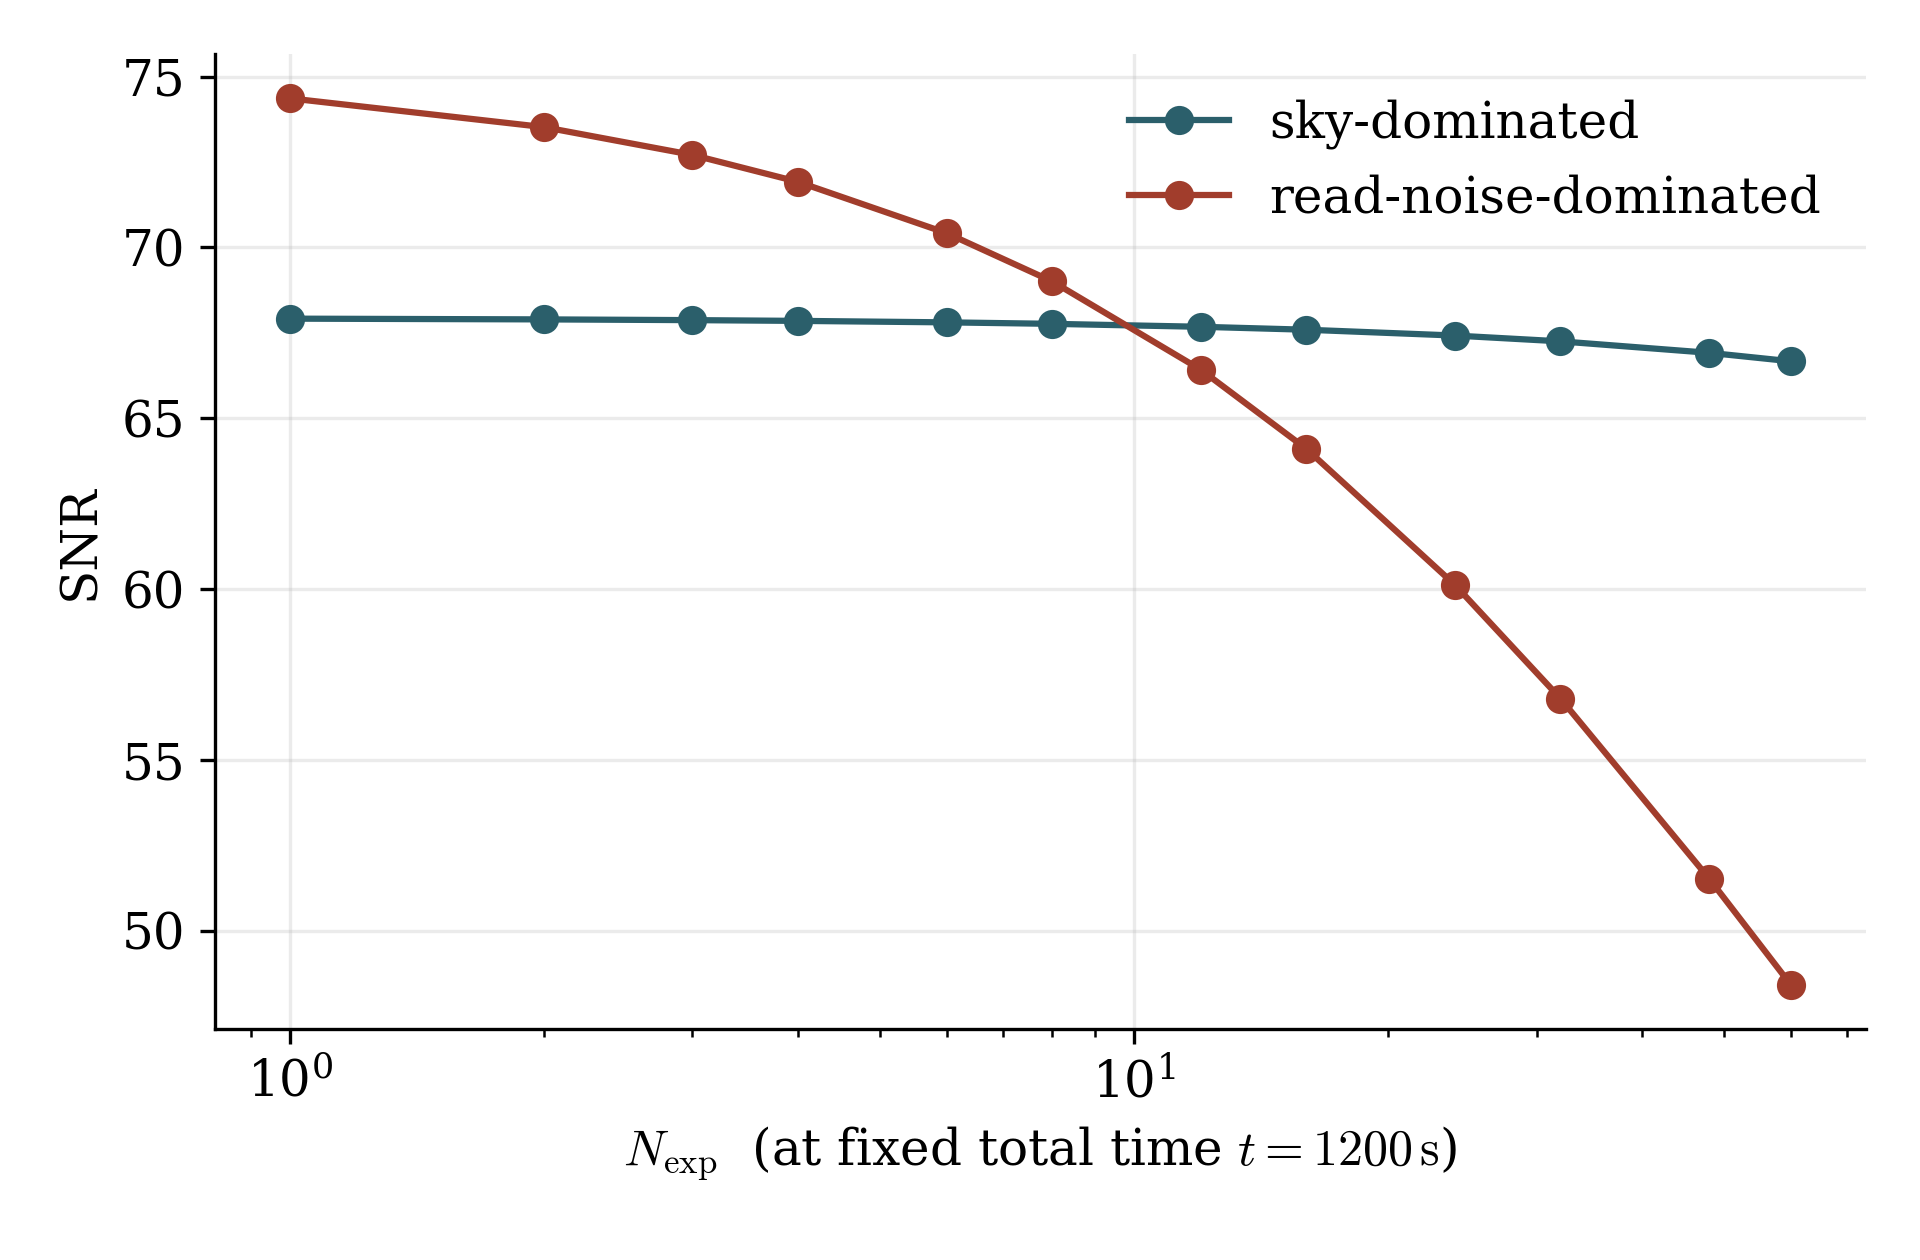
\includegraphics[width=0.85\textwidth]{figs/fig2_nexp.png}
\caption{SNR versus $N_{\rm exp}$ at \emph{fixed total exposure time} $t=N_{\rm exp}t_{\rm exp}=1200$\,s,
computed directly from the master equation (Eq.~\ref{eq:master}, no approximation) for two illustrative
parameter sets. \textbf{Sky-dominated} ($R_{\rm src}=50$, $R_{\rm sky}=30\ \mathrm{e^-s^{-1}pix^{-1}}$,
$n_{\rm pix}=20$, $\sigma_{\rm RON}=5\,\mathrm{e^-}$): the curve is essentially flat --- splitting the
exposure is nearly free. \textbf{Read-noise-dominated} ($R_{\rm src}=5$, $R_{\rm sky}=0.05$,
$n_{\rm pix}=6$, $\sigma_{\rm RON}=5\,\mathrm{e^-}$): SNR falls visibly as $N_{\rm exp}$ grows, because
each additional readout adds a fixed noise penalty unrelated to how much light was actually collected.
Same total integration time, same instrument-class read noise --- opposite conclusions about how to
schedule the exposure.}
\end{figure}


\FloatBarrier
\section*{Summary: reading the regime off the noise budget}

All three limits are the same equation; they differ only in which of four physically distinct terms
--- object shot noise, sky shot noise, dark shot noise, read noise --- happens to dominate the sum in
the denominator. That, and nothing more exotic, is why ``should I take one exposure or many?'' and
``should I bin?'' have different answers in different kinds of observations: the questions are really
asking which term in $\sigma_{\rm tot}^2$ you're fighting.

\begin{center}
\begin{tabular}{@{}l l l p{5.4cm}@{}}
\toprule
\textbf{Regime} & \textbf{Dominant term} & \textbf{SNR scaling} & \textbf{Strategy} \\
\midrule
Bright source & $\sigma_{\rm src}^2$ & $\sqrt{t}$ & watch for saturation, not SNR \\
Sky-limited & $\sigma_{\rm sky}^2$ & $\sqrt{t}/\sqrt{n_{\rm pix}}$ & splitting exposures is free; good seeing helps directly \\
Read-noise-limited & $\sigma_{\rm read}^2$ & $n_{\rm pix}^{-1/2}N_{\rm exp}^{-1/2}$ & bin pixels; keep $t_{\rm exp}$ as long as cosmic rays allow \\
\bottomrule
\end{tabular}
\end{center}

\vspace{18pt}
{\footnotesize\color{muted}
Physical content and worked numbers adapted from O.\ Hainaut, ``Signal, Noise and Detection'' (ESO,
2005); the notation, the units flag on dark current, and the figures above are this document's own.\par}

\end{document}
